% ======================================================================
% Inside the Machine — AAAI-style paper skeleton
%
% DRAFT STATUS (2026-08-19): converted from paper/01-intro.md and
% paper/02-system-and-ongoing.md, which were drafted by Claude at the
% author's direction. EVERY CLAIM requires author sign-off at the
% scheduled post-completion deep-dive before any submission. All
% [SIGN-OFF] / [FILL AT LAUNCH] / [VERIFY] markers from the drafts are
% preserved below as visible colored todo notes (\signoff, \fillatlaunch,
% \verifynote). Set \showtodosfalse to hide them; delete them entirely
% before submission.
%
% STYLE SWITCH: if the official AAAI author kit file aaai26.sty sits
% next to this file, it is used automatically (zero-line change). If the
% kit for the target year has a different name (e.g. aaai27.sty), edit
% the ONE marked line below. Without the kit, aaai-fallback.sty
% approximates the AAAI two-column geometry so the draft compiles
% anywhere. See README.md.
% ======================================================================

\newif\ifaaaikitpresent
\IfFileExists{aaai26.sty}{\aaaikitpresenttrue}{\aaaikitpresentfalse}  % <- ONE-LINE CHANGE for a different kit year

\ifaaaikitpresent
  % --- Official AAAI author kit path (kit conventions: do not change) ---
  \documentclass[letterpaper]{article}
  \usepackage[submission]{aaai26}  % camera-ready: drop the [submission] option
\else
  % --- Fallback path: no kit on this machine -----------------------------
  \documentclass[letterpaper,twocolumn]{article}
  \usepackage{aaai-fallback}
\fi

% --- AAAI author-kit required packages (kit forbids adding options) ----
\usepackage{times}
\usepackage{helvet}
\usepackage{courier}
\usepackage[hyphens]{url}
\usepackage{graphicx}
\urlstyle{rm}
\def\UrlFont{\rm}
\usepackage{natbib}   % AAAI kit requires natbib with no options
\usepackage{caption}
\frenchspacing
\ifdefined\pdfpagewidth
  \setlength{\pdfpagewidth}{8.5in}
  \setlength{\pdfpageheight}{11in}
\fi

% --- Draft-only: visible todo markers (NOT part of the AAAI kit) -------
% Strip this block and every \signoff/\fillatlaunch/\verifynote call
% before submission. xcolor is draft-only; the kit disallows extras.
\usepackage{xcolor}
\newif\ifshowtodos
\showtodostrue   % set \showtodosfalse for a clean read-through build
\ifshowtodos
  \newcommand{\signoff}[1]{{\color{red!75!black}\bfseries [SIGN-OFF: #1]}}
  \newcommand{\fillatlaunch}[1]{{\color{blue!70!black}\bfseries [FILL AT LAUNCH: #1]}}
  \newcommand{\verifynote}[1]{{\color{orange!80!black}\bfseries [VERIFY: #1]}}
\else
  \newcommand{\signoff}[1]{}
  \newcommand{\fillatlaunch}[1]{}
  \newcommand{\verifynote}[1]{}
\fi

% --- PDF metadata (AAAI camera-ready requirement; pdftex only) ---------
\ifdefined\pdfinfo
\pdfinfo{
/Title (Inside the Machine: An Interactive Guide to How LLMs Actually Think)
/Author (Shangyan Shen)
}
\fi

\title{Inside the Machine: An Interactive Guide to How LLMs Actually Think}
\author{Shangyan Shen}
\affiliations{Independent Researcher\\ shenshangyan2001@gmail.com}

\begin{document}

\maketitle

\begin{abstract}
Large language models are, by usage, among the most widely adopted
software artifacts of the decade --- and, for most of their users, the
least understood. \emph{Inside the Machine} is a long-form interactive
essay that lets a curious non-engineer put their own sentence into a
transparent model: every widget runs a complete GPT-Neo forward pass ---
under 250 lines of dependency-free TypeScript, verified token-exactly
against the reference implementation --- entirely in the reader's
browser tab, and every visualization (tokenization, an embedding map,
attention heads discovered live, next-token gambling, the
autoregressive loop) is computed from the reader's own words. The
narrative assumes no ML background and is fully bilingual
(English/Chinese). The essay, its Classroom Edition, and its engine are
open source (MIT) and archived on Zenodo
(DOI~10.5281/zenodo.22089051); the site launches at
\url{https://insidethemachine.org}. \fillatlaunch{switch ``launches
at'' to ``is at'' once the deploy is live}
\signoff{abstract; requires author approval like everything else}
\end{abstract}

\noindent\signoff{GLOBAL: drafted by Claude at the author's direction
(2026-08-19, finalized 2026-08-24); every claim requires author
sign-off at the read-through before any submission}

\section{Introduction}

Large language models are, by usage, the most widely adopted software
artifacts of the decade --- and, for most of their users, the least
understood. The prevailing mental models are either magic or dismissal
(``fancy autocomplete''), and both fail the same test: they give a
person no way to reason about \emph{why} the system just did what it
did. High-quality explainers exist, but each leaves a gap. The
most-cited introduction, \emph{The Illustrated Transformer}
\citep{alammar2018illustrated}, is static and speaks the field's
vocabulary (embeddings, encoder--decoder, softmax); Bycroft's 3D
walkthrough \citep{bycroft2023llmviz} renders a real network in
exquisite detail, for readers who already speak linear algebra; and
Transformer Explainer \citep{cho2025transformer}, the closest neighbor
to this work, puts a live GPT-2 in the browser but keeps its
computation inside a compiled inference runtime and its narrative in
English, couched in the field's terms.
The Annotated Transformer \citep{rush2018annotated} pioneered the
implementation-as-exposition ideal this work adopts, but as runnable
code for practitioners; CNN Explainer \citep{wang2021cnnexplainer}
established live in-browser visualization pedagogy for convolutional
networks. \signoff{previous sentence added during LaTeX conversion to
wire the Rush and Wang citations; approve wording} None of them lets a
curious non-engineer put \emph{their own sentence} into a
\emph{transparent} model and read, in plain language, what happens to
it.

\emph{Inside the Machine} is a long-form interactive essay built around
that missing experience. The reader types a sentence; that sentence
becomes the connective thread of seven acts --- it is chopped into
tokens, located on a map of meaning, watched by attention heads,
gambled on token by token, looped into generation, and finally used to
explain both what scale buys and why models confabulate. Every widget
runs a real model (GPT-Neo, TinyStories-1M, 7.5\,MB of fp16 weights
self-hosted as a static asset) entirely in the reader's browser tab;
nothing typed ever leaves the device. The narrative is written for
readers with no ML background and is fully bilingual (English/Chinese).
% original draft phrasing: (English / 中文)

This experience rests on two contributions:

\paragraph{C1 --- an auditable in-browser model.}
The essay's model is not an embedded inference runtime but a complete
GPT-Neo forward pass written in under 250 lines of dependency-free
TypeScript (tensor ops, the transformer stack, and a hand-rolled
safetensors parser --- 238 code lines; the full engine, adding weight
loading, sampling, embedding-neighbor search, and the live
attention-head diagnostics, is 501), executing in 5--20\,ms per pass
for typical sentences on a laptop. Its fidelity is enforced by a test
suite pinned to the reference implementation: a pinned prompt's greedy
12-token continuation must reproduce the reference token ids exactly,
and the leading last-position logits are checked against the reference
within fp16 tolerance, with the top next-token ranking required to
agree --- which required faithfully reimplementing GPT-Neo's
idiosyncratic departure from standard attention scaling (no
$1/\sqrt{d}$ division). Where prior in-browser explainers visualize
tensors emitted by an opaque compiled artifact, here the exposition and
the implementation are the same object: every number on screen is
traceable to source code a motivated reader can read.
\signoff{AUTHOR: this is the load-bearing differentiation vs.\
Transformer Explainer --- must be phrased exactly this carefully, and
the author must be able to defend it in review}

\paragraph{C2 --- the reader's own words as the pedagogy.}
No visualization in the essay is canned. The embedding map searches the
model's actual embedding table for the reader's word; the attention
room renders the model's actual attention tensors over the reader's
sentence, and \emph{automatically discovers} interpretable heads --- a
previous-token head, an anchor head, a most-diffuse head --- by
scanning those live tensors rather than presenting curated examples;
the probability bars and the autoregressive loop gamble on the reader's
own prefix. The essay's claim is that ``it computed THIS from MY
sentence'' is a categorically stronger teaching move than any
pre-rendered illustration, and the bilingual plain-language narration
extends it to audiences existing explainers do not reach.
\signoff{AUTHOR: pedagogical claim wording}

\paragraph{Status.}
The essay was released as open source in August~2026 (MIT; engine and
essay archived on Zenodo, DOIs 10.5281/zenodo.22089051 and
10.5281/zenodo.22089053) together with a Classroom Edition: the same
widgets packaged as two lesson modules with teacher guides, printables,
an unplugged activity, standards crosswalks, and a WCAG-audited,
offline-capable build. Three further essays in the series (on
confabulation, attention-head taxonomy, and tokenization failure modes)
are built and in editorial review, with a monthly cadence planned.
\fillatlaunch{deployment numbers for a future revision, once the
host-side counters have accumulated}

\begin{figure}[t]
  \centering
  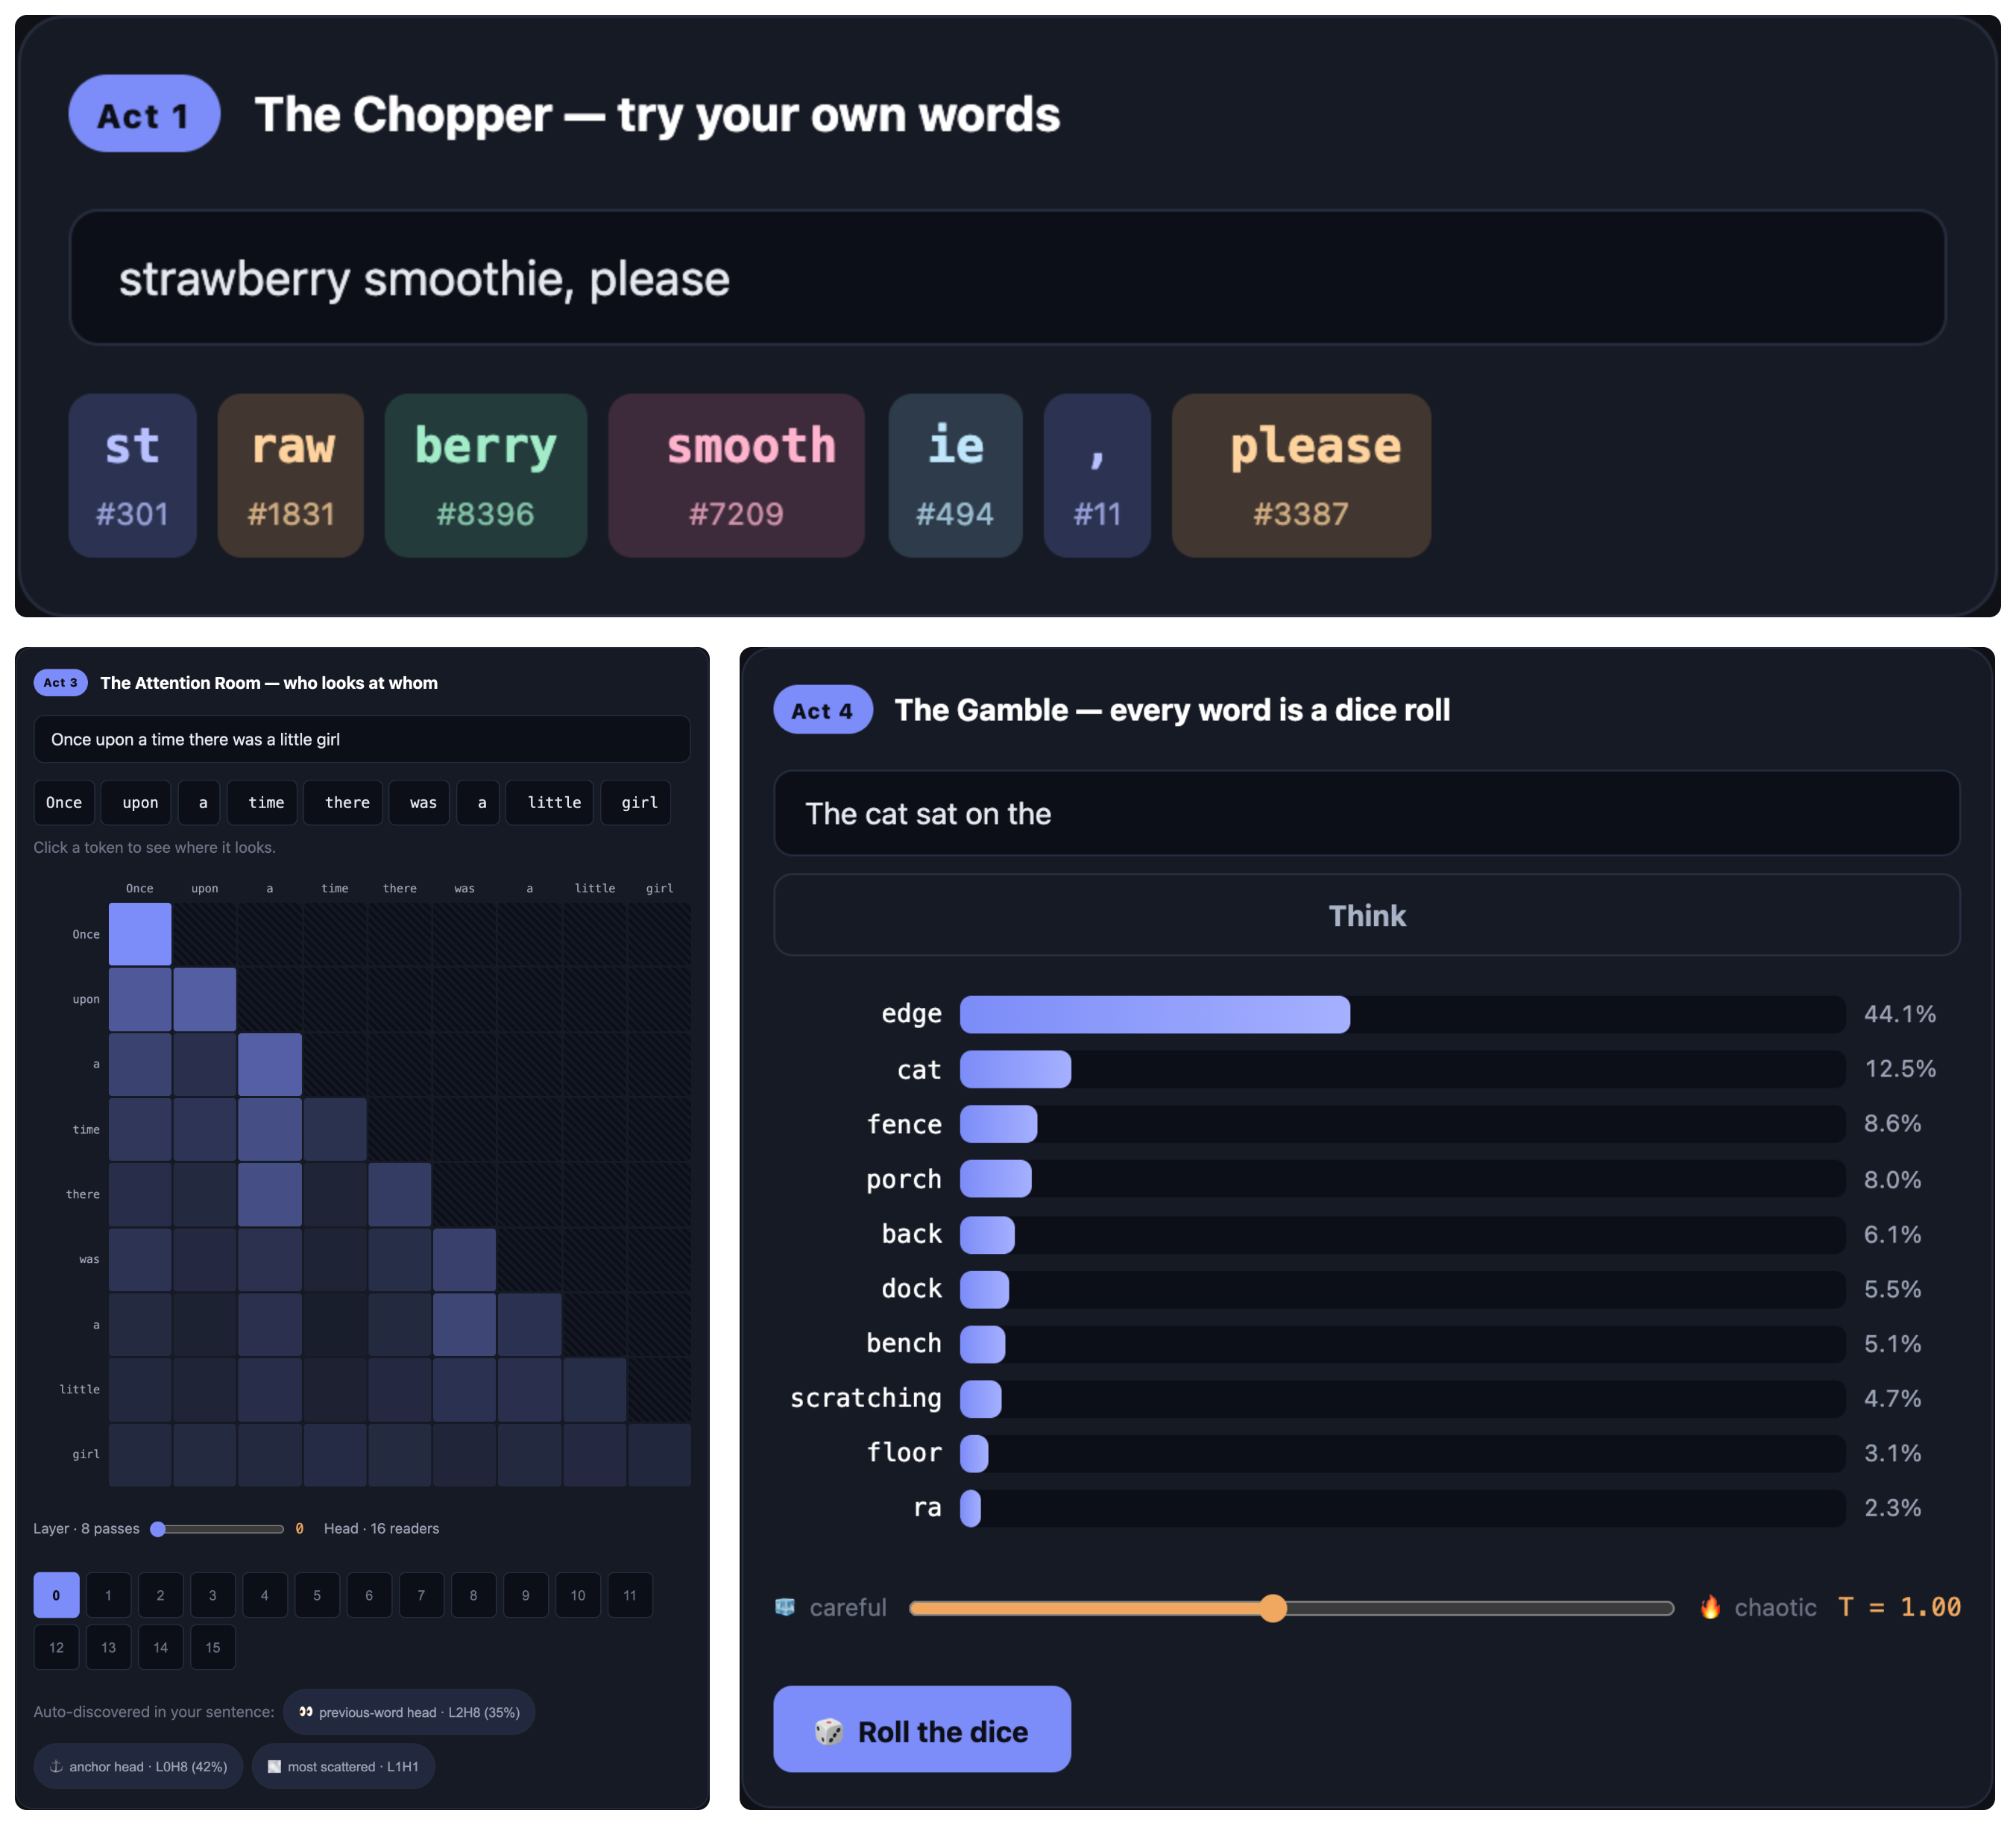
\includegraphics[width=\columnwidth]{figures/interface}
  \caption{The reader's sentence is the essay's connective thread.
  Top: the sentence fragments into tokens (Act 1). Bottom left: the
  attention room renders the model's live attention tensors over the
  reader's sentence and automatically discovers interpretable heads ---
  here a previous-token head at L2H8 and an anchor head at L0H8
  (Act 3). Bottom right: the probability bars gamble on the next token
  as the temperature slider moves (Act 4, the optional larger model).
  Every number shown is computed live in the browser tab.
  \signoff{caption}}
  \label{fig:interface}
\end{figure}

\section{System Design and Implementation}
% Draft note preserved from 02-system-and-ongoing.md header:
% "DRAFT — author sign-off required at the deep-dive"

Two principles shaped the essay.

\paragraph{P1 --- The implementation is the exposition.}
Every number the reader sees is produced by a forward pass they can
read: a dependency-free TypeScript implementation of GPT-Neo (238 code
lines covering the tensor ops, the transformer stack, and a hand-rolled
safetensors parser) running TinyStories-1M (7.5\,MB, fp16,
self-hosted). Fidelity is enforced as described in C1: a token-exact greedy
continuation and fp16-tolerance logit checks against the reference
implementation. \signoff{verification protocol wording}

\paragraph{P2 --- The reader's sentence is the curriculum.}
The seven acts follow the actual data path (tokenize $\rightarrow$
embed $\rightarrow$ attend $\rightarrow$ sample $\rightarrow$ loop),
and every visualization is computed live from the reader's own input.
The attention act discovers interpretable heads --- previous-token,
anchor, most-diffuse --- by scanning the live attention tensors of the
reader's sentence rather than showing curated examples. Act 4
optionally wakes a larger model (SmolLM2-135M-Instruct, 136\,MB
quantized, explicit click, cached) for richer next-token distributions.
The narrative is plain-language and fully bilingual (English/Chinese).
% original draft phrasing: (EN/中文)

\paragraph{Usage scenario.}
A high-school teacher pastes a sentence from tomorrow's lesson. She
watches it fragment into tokens (and sees why letter-counting fails),
finds the previous-token head reading HER sentence, drags the
temperature slider until the dice go wild, and steps the loop one
gamble at a time --- arriving at Act 7 already owning the explanation
of why the model confabulates. \signoff{scenario tone}

\paragraph{Implementation.}
React + Vite + TypeScript; ${\sim}10$\,ms per forward pass on a laptop;
everything runs client-side with zero telemetry --- typed text never
leaves the tab.

\section{Ongoing Work}

The series continues at a planned monthly cadence (three essays are in
editorial review), and the Classroom Edition moves from materials to
classroom pilots with instructors other than the author. Deployment
counting stays host-side (static-host request statistics, no in-page
analytics), keeping the essay's ``nothing you type leaves the tab''
promise intact while still producing the usage evidence an extended
paper needs. Planned next: instructor outreach (the essay is designed
as assignable course reading) and a formal learning-outcome study.
\signoff{ongoing-work framing}

\section*{Acknowledgments}
This system and manuscript were developed with substantial assistance
from an AI assistant (Claude), directed and reviewed by the author, who
takes full responsibility for all content. \signoff{AI-assistance
disclosure wording --- consistent with the repository's public
Co-Authored-By commit trailers}

% Optional future reference noted in the draft: Olah et al.,
% distill.pub lineage for "explorable explanations". Add to
% references.bib if the author signs off on citing it.
\ifaaaikitpresent
  \bibliographystyle{aaai26}  % requires aaai26.bst next to this file
\else
  \bibliographystyle{plainnat}
\fi
\bibliography{references}

\end{document}
